\textcolor{ubuntu_orange}{Empathy} jest wbudowanym w Ubuntu komunikatorem internetowym obsługującym różne protokoły sieciowe. Domyślnie Empathy korzysta z systemowej obsługi \textcolor{ubuntu_orange}{Konta Sieciowe} w celu nawiązywania rozmów.

Poza usługami z którymi możesz się połączyć przez Konta Sieciowe obsługuje protokoły Jabbera, AIM, Gadu-Gadu, GroupWize, ICQ, IRC, MSN (Windows Live) i inne.

\subsubsection{Sterowanie Empathy}
Empathy można sterować za pomocą ikony 
\includegraphics{images/unity_wskaznik_wiadomosci.png} umieszczonego w pasku menu. Wskaźnik zmieni kolor na niebieski jeżeli są jakieś nieprzeczytane wiadomości. Kliknięcie na ten wskaźnik otworzy menu z możliwością zmiany statusu (np. dostępny, niewidoczny, zajęty, rozłączony) a także wyświetli ewentualne rozpocząte, ale nieprzeczytane rozmowy. Pozycja \textcolor{ubuntu_orange}{Empathy} uruchamia główne okno programu, zawierające twoich znajomych.

\subsubsection{Przykładowa konfiguracja konta Gadu-Gadu}
\begin{enumerate}
\item W dashu wyszukaj i uruchom \textcolor{ubuntu_orange}{empathy-accounts}.
\item Zostaniesz poproszony o wpisanie swoich danych do komunikacji wewnątrz sieci lokalnej. Możesz pominać ten krok.
\item Pod lewym panelem znajduje się przycisk \textcolor{ubuntu_orange}{+}. kliknij go.
\item \begin{minipage}[t]{\linewidth}
          \raggedright
          \adjustbox{valign=t}{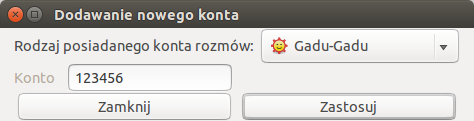
\includegraphics[width=.8\linewidth]{images/programy_empathy1.png}}
          
          \medskip
          Z rozwijanej listy wybierz \textcolor{ubuntu_orange}{Gadu-Gadu}. W pole \textcolor{ubuntu_orange}{Konto} wpisz swój numer w sieci GG a następnie kliknij \textcolor{ubuntu_orange}{Zastosuj}
    \end{minipage}
\item Konto zostanie dodane. Wybierz \menu{{Modyfikuj parametry połączenia}>{Zaawansowane}} i wpisz swoje hasło. Kliknij na \textcolor{ubuntu_orange}{Zastosuj} aby zapisać hasło.
\item Połączenie z Gadu-Gadu jest gotowe.
\end{enumerate}